\documentclass[11pt,a4paper,openany]{report}

\usepackage[utf8]{inputenc}
\usepackage[T1]{fontenc}
\usepackage{lmodern}
\usepackage{geometry}
\usepackage{hyperref}
\usepackage{graphicx}
\usepackage{listings}
\usepackage{xcolor}
\usepackage{enumitem}
\usepackage{booktabs}
\usepackage{multirow}
\usepackage{amssymb}
\usepackage{amsmath}
\usepackage{pifont}
\usepackage{float}
\usepackage{tcolorbox}
\usepackage{tabularx}
\usepackage{longtable}
\usepackage{array}
\usepackage{caption}
\usepackage{xurl}

\makeatletter
\renewcommand\chapter{\@startsection{chapter}{0}{\z@}%
  {-3.5ex \@plus -1ex \@minus -.2ex}%
  {2.3ex \@plus .2ex}%
  {\normalfont\Huge\bfseries}}
\makeatother

\geometry{margin=1in}
\hypersetup{
  colorlinks=true,
  linkcolor=blue,
  urlcolor=blue,
  pdftitle={ARIA: AI-Assisted Forensic Investigation Game},
  pdfauthor={Renato Mignone},
  pdfsubject={Computer Forensics and Cyber Crime Analysis - Serious Game Report},
  pdfkeywords={computer forensics, serious game, AI hallucination, digital evidence, forensic training}
}

\graphicspath{{resources/images/}}
\setlength{\parskip}{0.45em}
\setlength{\parindent}{0pt}
\renewcommand{\arraystretch}{1.18}
\newcolumntype{Y}{>{\raggedright\arraybackslash}X}

\title{ARIA: AI-Assisted Forensic Investigation Game}
\author{Renato Mignone}
\date{June 2026}

\begin{document}

\hypersetup{pageanchor=false}
\begin{titlepage}
  \centering
  \vspace*{0.5cm}
  
\includegraphics[width=0.4\textwidth]{resources/images/polito_logo.png}

  \vspace{1.5cm}
  {\LARGE Politecnico di Torino \par}
  \vspace{0.4cm}
  {\large Computer Forensics and Cyber Crime Analysis \par}

  \vspace{1.2cm}
  {\LARGE\bfseries ARIA: AI-Assisted Forensic Investigation Game\par}
  \vspace{0.4cm}
  {\large Serious Game Report\par}

  \vspace{1.5cm}
  {\Large\bfseries Renato Mignone\par}
  \vspace{0.2cm}
  {\large Matricola: s336973\par}

  \vfill
  {\large June 2026\par}
\end{titlepage}
\hypersetup{pageanchor=true}
\pagenumbering{roman}
\begingroup
\small
\setlength{\parskip}{0pt}
\tableofcontents
\endgroup
\clearpage
\pagenumbering{arabic}

\chapter*{Abstract}
\addcontentsline{toc}{chapter}{Abstract}

ARIA is a browser-based serious game developed for the Computer Forensics and Cyber Crime Analysis course. The player acts as a forensic investigator assigned to a simulated business email compromise and corporate fraud case involving an unauthorized EUR 2.3M wire transfer. During the investigation, the player examines five digital evidence artifacts, questions an AI assistant, validates AI-generated claims, connects related evidence, and submits a final report.

The central educational objective is to train \textbf{calibrated trust} in AI-assisted investigative workflows. ARIA is intentionally useful but unreliable: it provides both correct observations and plausible hallucinations. The game therefore converts the abstract warning that ``AI can be wrong'' into an operational exercise where each AI claim must be accepted or rejected only after inspecting raw evidence such as email headers, media metadata, PDF metadata, hashes, timestamps, and network logs.

The current prototype is implemented as a React and TypeScript single-page application. It supports deterministic scripted gameplay for classroom evaluation and an optional local Gemini-backed mode for experimentation. The main contribution of the project is a complete \textbf{evidence-first} game loop: inspect, ask, verify, connect, report, and debrief.

\chapter{Context and Problem Statement}

\section{Project Context}

ARIA, short for AI-Assisted Research and Investigation Assistant, is a serious game about digital forensics and AI reliability. The player is placed in the role of an analyst investigating a corporate fraud incident at TechCorp. The case combines email spoofing, social engineering, synthetic audio, deepfake-style video indicators, suspicious invoice metadata, and network activity.

The project was developed as an individual extended homework for the Computer Forensics and Cyber Crime Analysis course. Its goal is not to replace a forensic suite, but to create a focused training environment where students practice the mental discipline required when AI tools are introduced into an investigation.

\section{Project Availability}

The public repository and hosted build are available at:

\begin{itemize}[leftmargin=*]
  \item Repository: \url{https://github.com/RenatoMignone/ARIA_Computer_Forensics_Game}
  \item Hosted game: \url{https://renatomignone.github.io/ARIA_Computer_Forensics_Game/}
\end{itemize}

\section{Why This Game Exists}

In 2026, large language models and AI agents are no longer exotic tools. They are used to summarize documents, interpret logs, draft incident reports, explain metadata, generate investigation leads, and automate small technical tasks. This makes them attractive in digital forensics because they can reduce friction and help a student move through unfamiliar evidence faster.

The problem is that the same fluency that makes these systems useful also makes their mistakes dangerous. An AI assistant can produce a confident explanation, invent a missing detail, invert a technical finding, or connect two artifacts more strongly than the evidence allows. In normal productivity work this may be annoying; in a forensic setting it can break \textbf{traceability}, damage the final report, or turn speculation into an apparently authoritative conclusion.

ARIA exists to train the habit that modern analysts increasingly need: use AI for assistance, but do not outsource judgment to it. The game lets the player experience the convenience of AI support while forcing every important statement back through raw evidence. In this sense, the player is not learning only about one TechCorp fraud case; they are practicing how to remain professionally skeptical when AI systems are embedded in everyday investigative work.

\section{Educational Gap}

Computer forensics teaching often separates individual technical skills: reading email headers, checking file metadata, interpreting logs, or reconstructing a timeline. These exercises are useful, but an investigation also requires connecting many small observations into a defensible conclusion. A second challenge is more recent: students are increasingly exposed to AI assistants that can summarize evidence, suggest leads, and draft explanations, but can also fabricate details while sounding precise.

ARIA addresses this gap by joining the two problems. It asks the player to perform a complete mini-investigation while an AI assistant gives both supported and unsupported statements. The intended habit is simple: AI can accelerate analysis, but evidence decides what enters the final report.

\section{Forensic Risk}

In a forensic context, an unsupported AI statement is not just a minor mistake. It can produce wrong attribution, inaccurate timelines, misread metadata, or conclusions that cannot be defended. A report based on confident but unverified language may look coherent while failing the basic requirement of \textbf{traceability to artifacts}.

The game therefore focuses on the risk of \textbf{AI overtrust}. It also avoids the opposite simplification: the correct lesson is not to reject every AI output automatically. Some AI claims are true and should be verified. The player is rewarded for calibrated judgment, not cynicism.

\section{Guiding Question}

The design question behind the project is:

\begin{quote}
How can an interactive game teach students to use AI support critically while preserving evidence-based forensic reasoning?
\end{quote}

ARIA answers through a claim-validation loop. The player inspects evidence, asks ARIA for analysis, validates individual claim badges as either verified or hallucinated, identifies cross-evidence links, and submits a final report that is evaluated in a debrief.

\chapter{Solution Design}

\section{Core Idea}

ARIA is built around one rule: AI may assist the investigation, but every conclusion must be verified against evidence. The assistant is presented as useful enough to be tempting, yet unreliable enough that blind trust is punished. The game mechanics are therefore not decorative; they create situated practice around the learning objective.

The game translates this principle into individual \textbf{claim badges}. Instead of asking the player to judge an entire AI paragraph, ARIA tags checkable statements such as \texttt{CLAIM-001}. Each claim has a stored ground truth, a related evidence artifact, feedback, a hint, and relevant metadata fields. This makes AI reliability measurable inside the gameplay loop.

\section{Main Gameplay Loop}

The investigation follows a repeated evidence-first pattern:

\begin{enumerate}[leftmargin=*]
  \item Select an evidence file from the vault.
  \item Inspect its visible content and raw metadata.
  \item Ask ARIA a focused forensic question.
  \item Read the generated claim badges.
  \item Validate each claim as \texttt{verified} or \texttt{hallucination}.
  \item Record confidence and notes.
  \item Connect related evidence when a shared artifact is found.
  \item Submit the final report and review the debrief.
\end{enumerate}

\section{Interface Flow}

The interface is designed to make the player enter the activity as an investigator rather than as a generic quiz participant. The main menu frames ARIA as an AI-assisted evidence review tool and immediately establishes the central theme of the game: the machine is useful, but it must not be trusted blindly.

\begin{figure}[H]
  \centering
  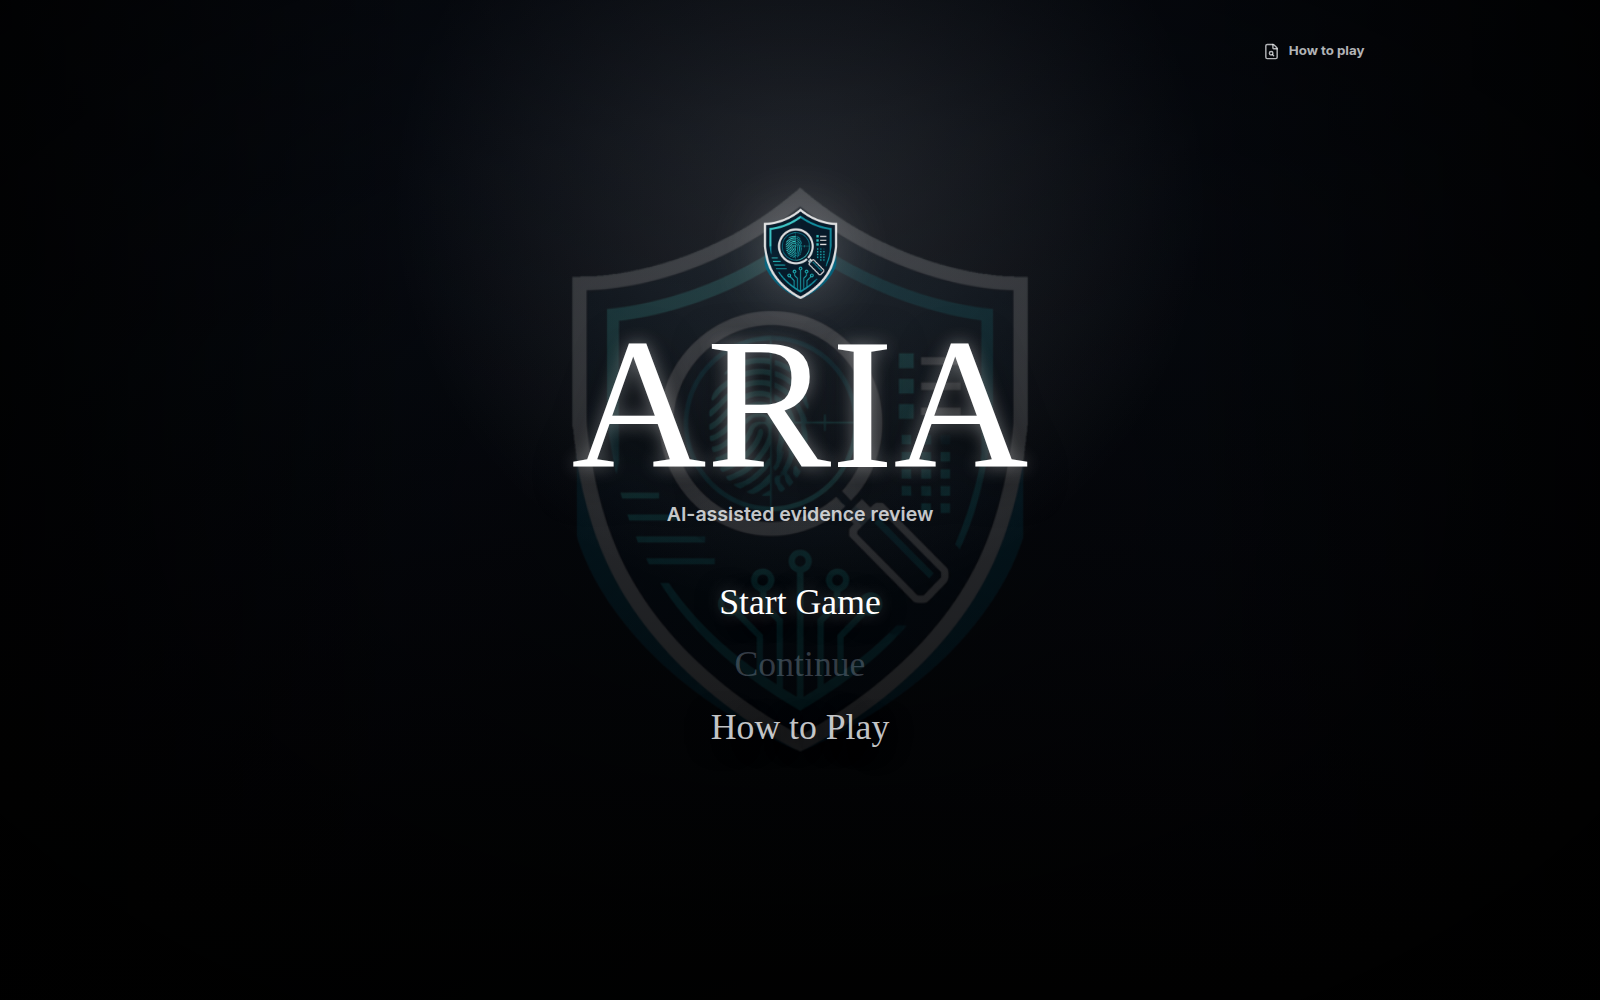
\includegraphics[width=0.96\textwidth]{aria_main_menu.png}
  \caption{ARIA main menu and case framing.}
  \label{fig:main-menu}
\end{figure}

Before the investigation starts, the player selects a game mode and then chooses whether to enable a timer. This separation is intentional: difficulty changes the information available to the player, while the timer changes the pressure under which the same forensic reasoning must be performed. The menu therefore presents assessment constraints before the case begins, instead of changing them silently during play.

\begin{figure}[H]
  \centering
  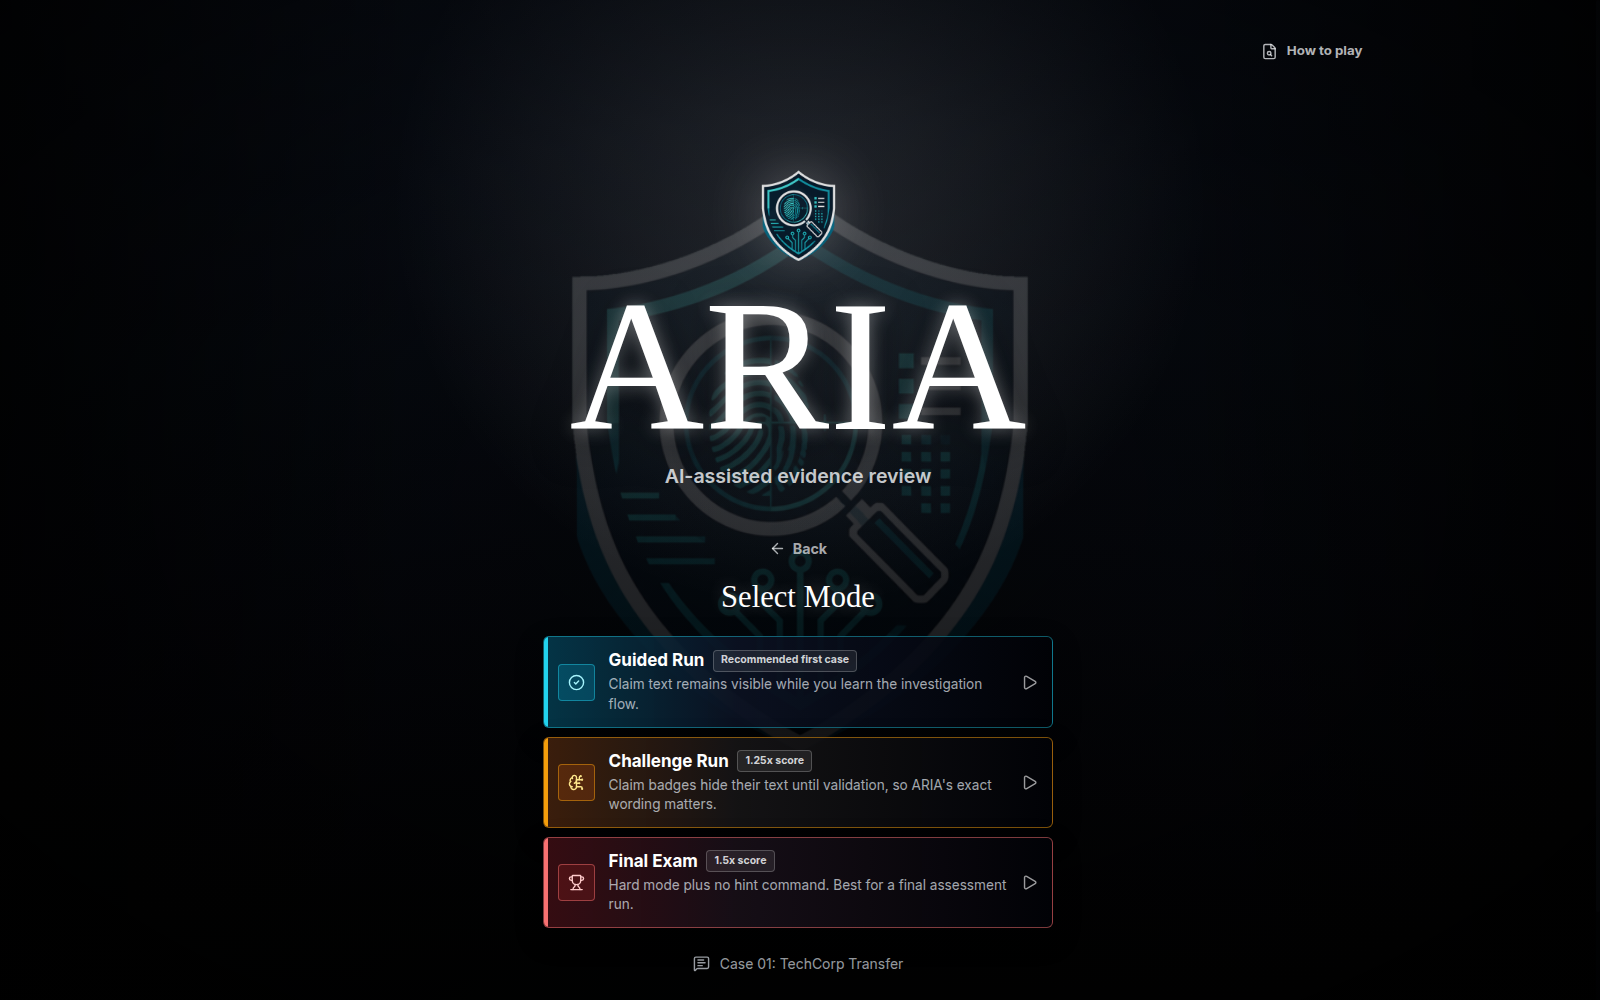
\includegraphics[width=0.96\textwidth]{aria_mode_selection.png}
  \caption{Difficulty selection screen used before starting the investigation.}
  \label{fig:mode-selection}
\end{figure}

\section{Game Modes}

The prototype supports three difficulty modes, shown in Table~\ref{tab:difficulty}.

\begin{table}[H]
\centering
\caption{Difficulty modes}
\label{tab:difficulty}
\begin{tabularx}{\textwidth}{lllY}
\toprule
Mode & Internal value & Multiplier & Purpose \\
\midrule
Guided Run & \texttt{standard} & 1.00 & Recommended first run; claim text remains visible while pending. \\
Challenge Run & \texttt{hard} & 1.25 & Claim text is hidden until validation, increasing reliance on evidence review. \\
Final Exam & \texttt{expert} & 1.50 & Hard mode with no hint command, intended for assessment-style play. \\
\bottomrule
\end{tabularx}
\end{table}

The negative values are intentionally asymmetric. Accepting a hallucination is the most dangerous failure because it lets an unsupported statement enter the investigation as fact. Rejecting a true claim is also penalized heavily, however, because the learning goal is \textbf{calibrated trust}, not automatic distrust. In the scripted scenario, this prevents a simple exploit where the player marks every AI statement as hallucinated and still obtains a good result.

Players may also choose a 45-minute timer, a 30-minute timer, or no timer. Finishing before an active timer expires grants a speed bonus.

\begin{figure}[H]
  \centering
  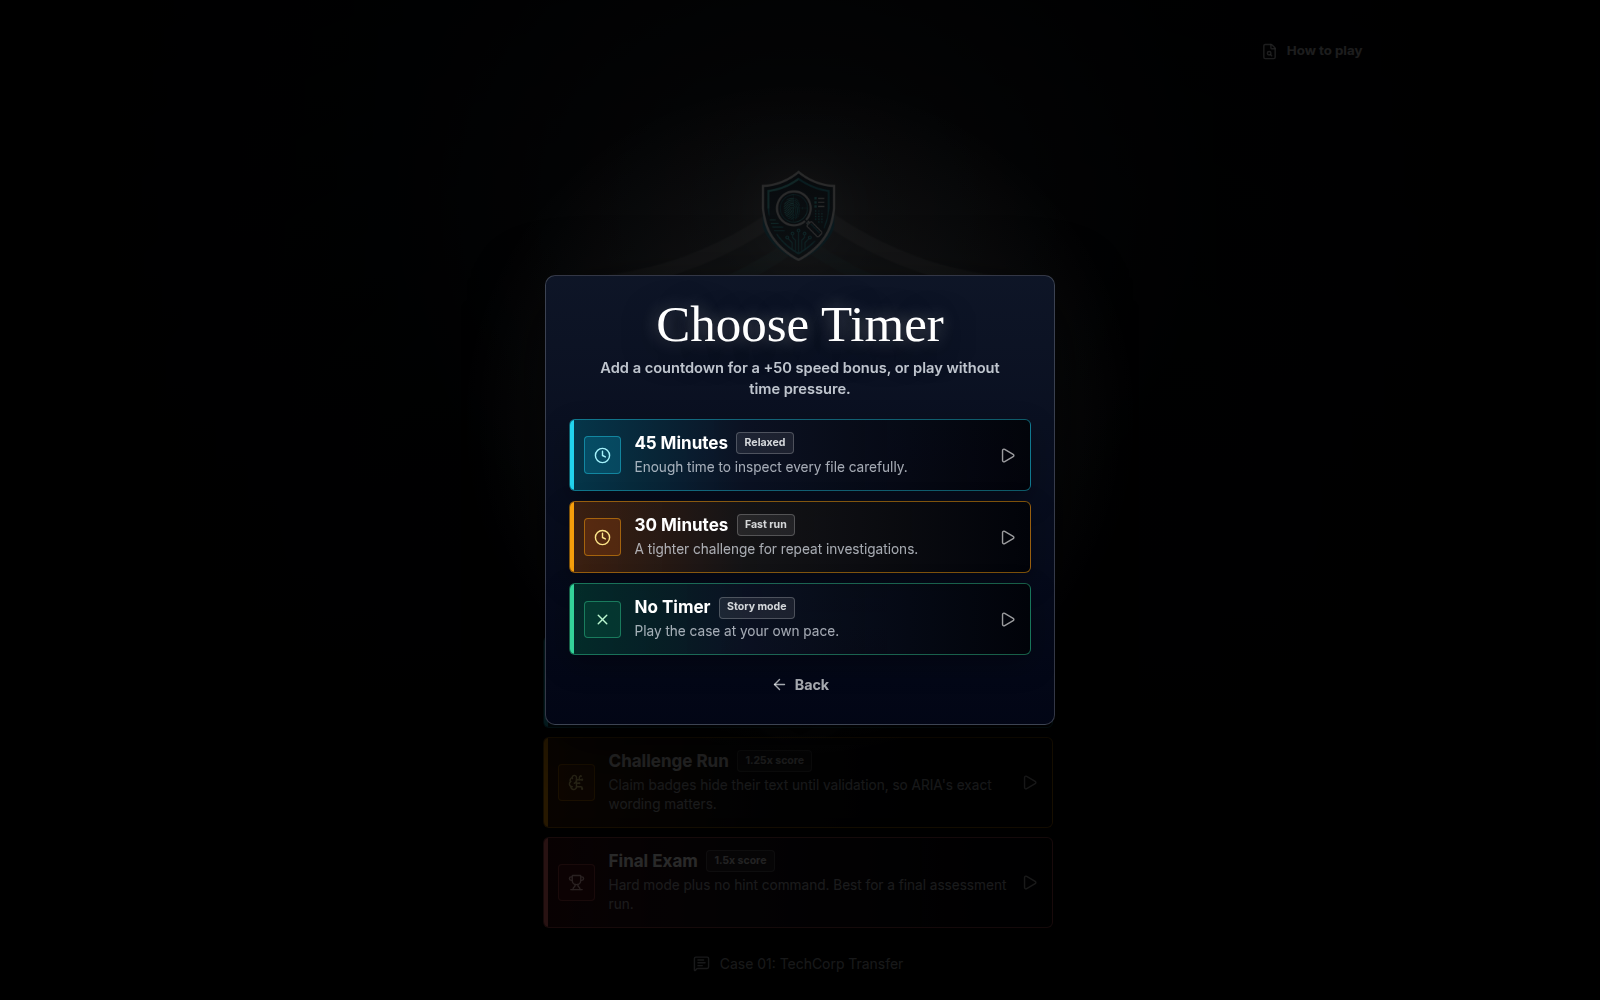
\includegraphics[width=0.96\textwidth]{aria_timer_choice.png}
  \caption{Timer choice prompt: optional pressure is configured separately from difficulty.}
  \label{fig:timer-choice}
\end{figure}

\section{Evidence Review Gate}

The most important safeguard is the \textbf{evidence review gate}. A claim cannot be validated until the related evidence has been reviewed through the terminal with commands such as \texttt{inspect}, \texttt{cat}, \texttt{strings}, \texttt{grep}, or \texttt{hash verify}. This prevents a weak strategy where the player only asks ARIA questions and clicks claim verdicts without touching the artifacts.

This mechanic aligns the interface with the learning objective. The scoring system does not merely ask whether the player knows the correct answer; it requires interaction with the source material before accepting or rejecting AI output.

\section{Scoring Model}

The score rewards correct verification and penalizes both blind trust and blanket rejection. The main scoring events are listed in Table~\ref{tab:scoring}.

\begin{table}[H]
\centering
\caption{Scoring events}
\label{tab:scoring}
\begin{tabularx}{\textwidth}{Yr}
\toprule
Action & Points \\
\midrule
Correctly flag a hallucination & +20 \\
Correctly verify a true claim & +10 \\
Accept a hallucination as true & -30 \\
Reject a true claim as hallucinated & -25 \\
Find a cross-evidence connection & +15 for each of the first 3 \\
Trace the Tor exit-node IP in the terminal & +15 once \\
Decode the hidden invoice creator payload & +20 once \\
Use a hint & -5 \\
Submit the final report & +50 \\
Submit before the timer expires & +50 \\
\bottomrule
\end{tabularx}
\end{table}

\chapter{Scenario and Learning Outcomes}

\section{Case Summary}

The scenario concerns an unauthorized EUR 2.3M wire transfer at TechCorp. The attacker appears to impersonate Marco Rossi, the company's CEO, and pressures Luca Ferrari, the CFO, to process an urgent payment. The incident is intentionally designed as a plausible \textbf{multi-artifact fraud}: the visible story seems coherent, but the underlying metadata reveals inconsistencies and signs of manipulation.

\section{Evidence Set}

The current game contains five evidence artifacts. Their forensic role is summarized in Table~\ref{tab:evidence}.

\begin{longtable}{p{0.22\textwidth}p{0.18\textwidth}p{0.50\textwidth}}
\caption{Scenario evidence set}
\label{tab:evidence}\\
\toprule
File & Type & Forensic purpose \\
\midrule
\endfirsthead
\toprule
File & Type & Forensic purpose \\
\midrule
\endhead
\texttt{email\_1.eml} & Email & Spoofed executive payment request. Relevant fields include SPF failure, DKIM domain mismatch, suspicious Return-Path, originating IP \texttt{91.200.81.47}, and high spam/phishing indicators. \\
\texttt{audio\_call.mp3} & Audio & Synthetic voice call. Metadata includes a creation timestamp at \texttt{2026-03-03T02:14:33Z}, 22050 Hz sample rate, TTS-like encoder traces, and synthetic background noise. \\
\texttt{teams\_meeting.mp4} & Video & Purported CEO confirmation call. Indicators include OBS Studio encoder metadata, missing GPS value, bitrate anomalies around the facial region, thumbnail mismatch, and compression artifacts. \\
\texttt{invoice\_fraud.pdf} & PDF & Suspicious invoice matching the requested amount and IBAN. Metadata shows AutoDoc AI Writer, no digital signature, short modification interval, and a base64-encoded creator field. \\
\texttt{network\_logs.txt} & Log & Firewall activity connecting an unregistered workstation to suspicious infrastructure, including \texttt{91.200.81.47}, Tor-related endpoints, and anomalous outbound traffic. \\
\bottomrule
\end{longtable}

\section{Cross-Evidence Reasoning}

The scenario is not solved by a single artifact. The player must connect multiple observations:

\begin{itemize}[leftmargin=*]
  \item The IP address \texttt{91.200.81.47} appears in both the email headers and the network logs.
  \item The audio creation timestamp aligns with suspicious outbound activity around 02:14 UTC.
  \item The invoice creation and modification times are close to outbound activity from an unregistered workstation.
\end{itemize}

These links teach a careful distinction between correlation and proof. For example, a shared IP address can support infrastructure correlation, but it should not be overclaimed as a definitive identity attribution unless the evidence supports that conclusion.

\section{AI Hallucination Model}

ARIA's scripted scenario contains 7 assistant responses and 28 unique claims. The claim set is intentionally balanced: \textbf{14 true claims and 14 hallucinated claims}. This avoids two bad lessons. If every claim were false, the player would learn to reject ARIA automatically. If every claim were true, the player would learn blind trust.

The hallucinations are grouped into recurring failure modes:

\begin{itemize}[leftmargin=*]
  \item \textbf{False attribution:} assigning authorship or responsibility without enough evidence.
  \item \textbf{Fabricated metadata:} inventing fields or observations not present in the artifact.
  \item \textbf{Inverted finding:} stating the opposite of the raw evidence.
  \item \textbf{Timestamp error:} misreporting or misinterpreting time evidence.
  \item \textbf{Confidence inflation:} making a strong claim without a defensible method.
\end{itemize}

\section{Learning Outcomes}

After playing, a successful student should be able to explain which AI claims were supported, which were hallucinated, and which artifacts justified each decision. The intended skills include reading email authentication fields, inspecting media and PDF metadata, checking hashes, interpreting firewall logs, comparing timestamps, constructing a simple incident timeline, and producing a defensible final report.

The broader professional habit is evidence discipline: use AI as a lead generator, not as an authority.

\chapter{Technical Implementation}

\section{Technology Stack}

ARIA is implemented as a browser-based single-page application. The main technologies are:

\begin{itemize}[leftmargin=*]
  \item React 19 and TypeScript 5.9 for the application logic and UI.
  \item Vite 7 for development, bundling, and static deployment.
  \item Tailwind CSS 4 for styling.
  \item xterm.js for the in-game forensic terminal.
  \item Framer Motion for interface transitions.
  \item Lucide React for icons.
  \item Optional Google Gemini integration for local live AI mode.
\end{itemize}

\section{Main Application Components}

The interface is organized into several panels and screens:

\begin{itemize}[leftmargin=*]
  \item The boot sequence, main menu, difficulty selection, timer selection, and tutorial introduce the case.
  \item The evidence vault lists case files and shows investigation progress.
  \item The workspace displays selected evidence, raw metadata, notes, and claim references.
  \item The ARIA chat panel returns scripted or live AI responses with claim badges.
  \item The terminal supports command-style investigation actions.
  \item The evidence board and attack timeline help the player reason across artifacts.
  \item The debrief screen reports score, errors, hallucinations found, calibration, and exportable report details.
\end{itemize}

The scenario is mostly \textbf{data-driven}. Evidence artifacts, scripted ARIA responses, claim truth labels, hints, feedback, valid cross-evidence links, and timeline feedback are stored as structured project data. This keeps the case content inspectable and makes future scenario expansion possible without rewriting the interface.

Figure~\ref{fig:workspace-initial} shows the initial investigation workspace after selecting the email evidence. The layout keeps three investigation surfaces visible at the same time: the evidence vault on the left, the file content and metadata in the center, and the ARIA chat on the right. The terminal is kept at the bottom because it represents the raw-evidence workflow that the player must use before a claim can be accepted or rejected.

\begin{figure}[H]
  \centering
  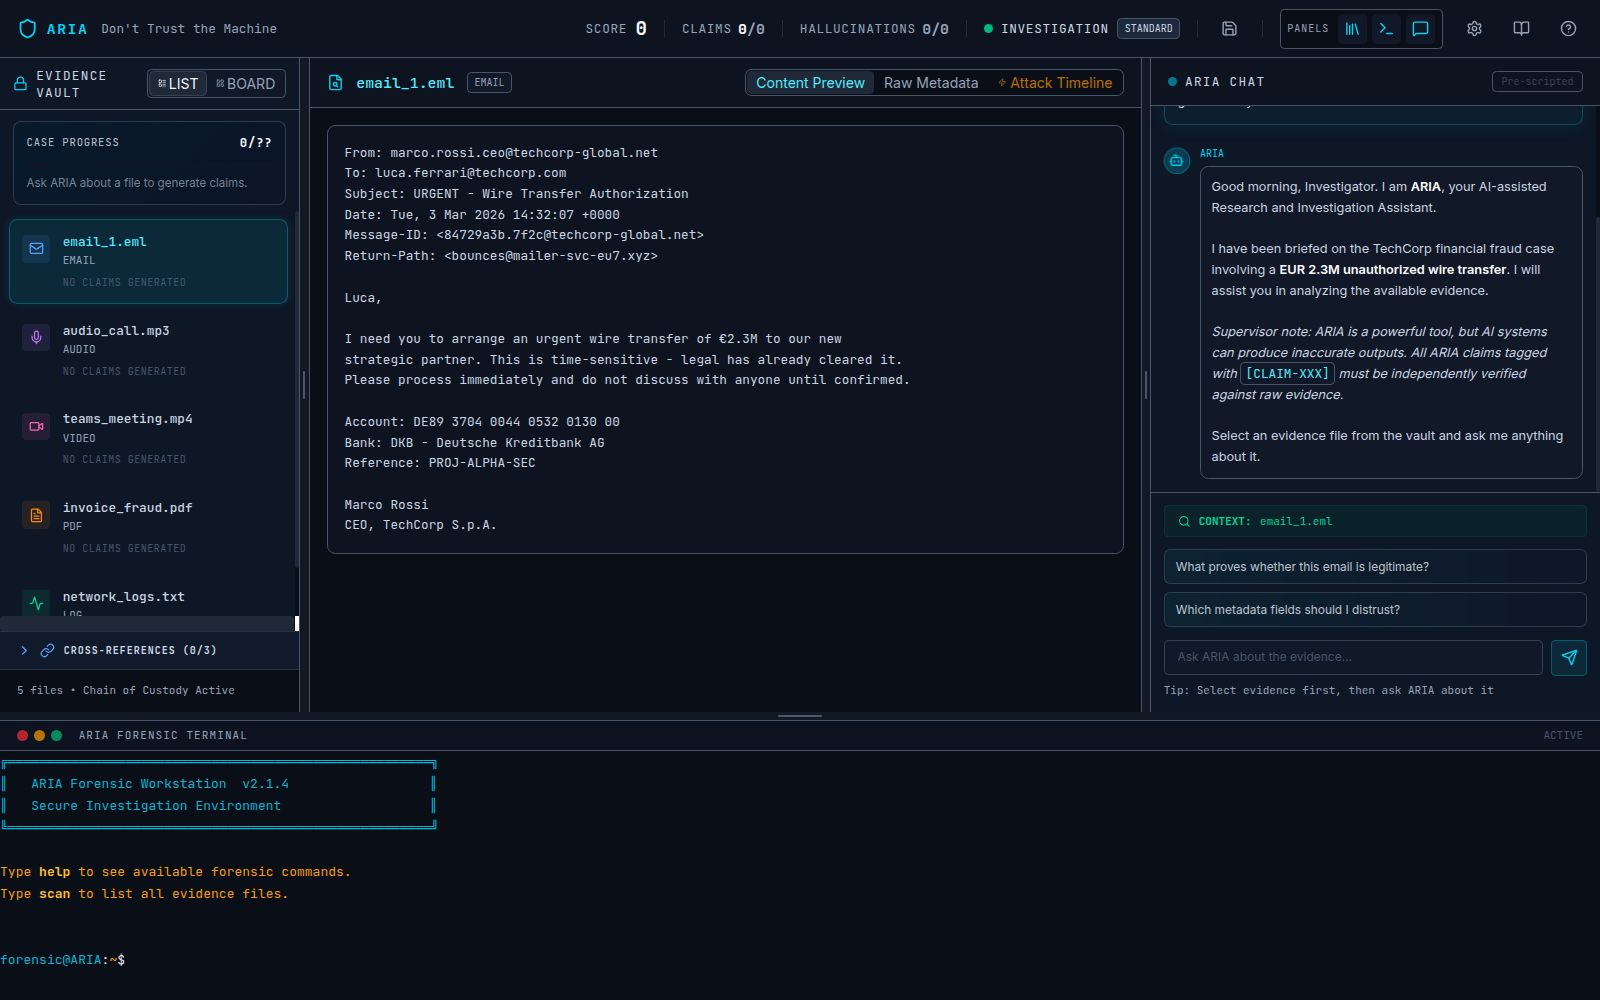
\includegraphics[width=0.96\textwidth]{aria_workspace_initial.png}
  \caption{Investigation workspace after selecting the first evidence file.}
  \label{fig:workspace-initial}
\end{figure}

Figure~\ref{fig:claim-review} shows the same workspace after ARIA has generated claim badges. The claim list is deliberately placed next to the raw metadata panel rather than inside a separate quiz screen. This reinforces the intended behavior: every AI statement is judged only after the player has compared it with the underlying artifact.

\begin{figure}[H]
  \centering
  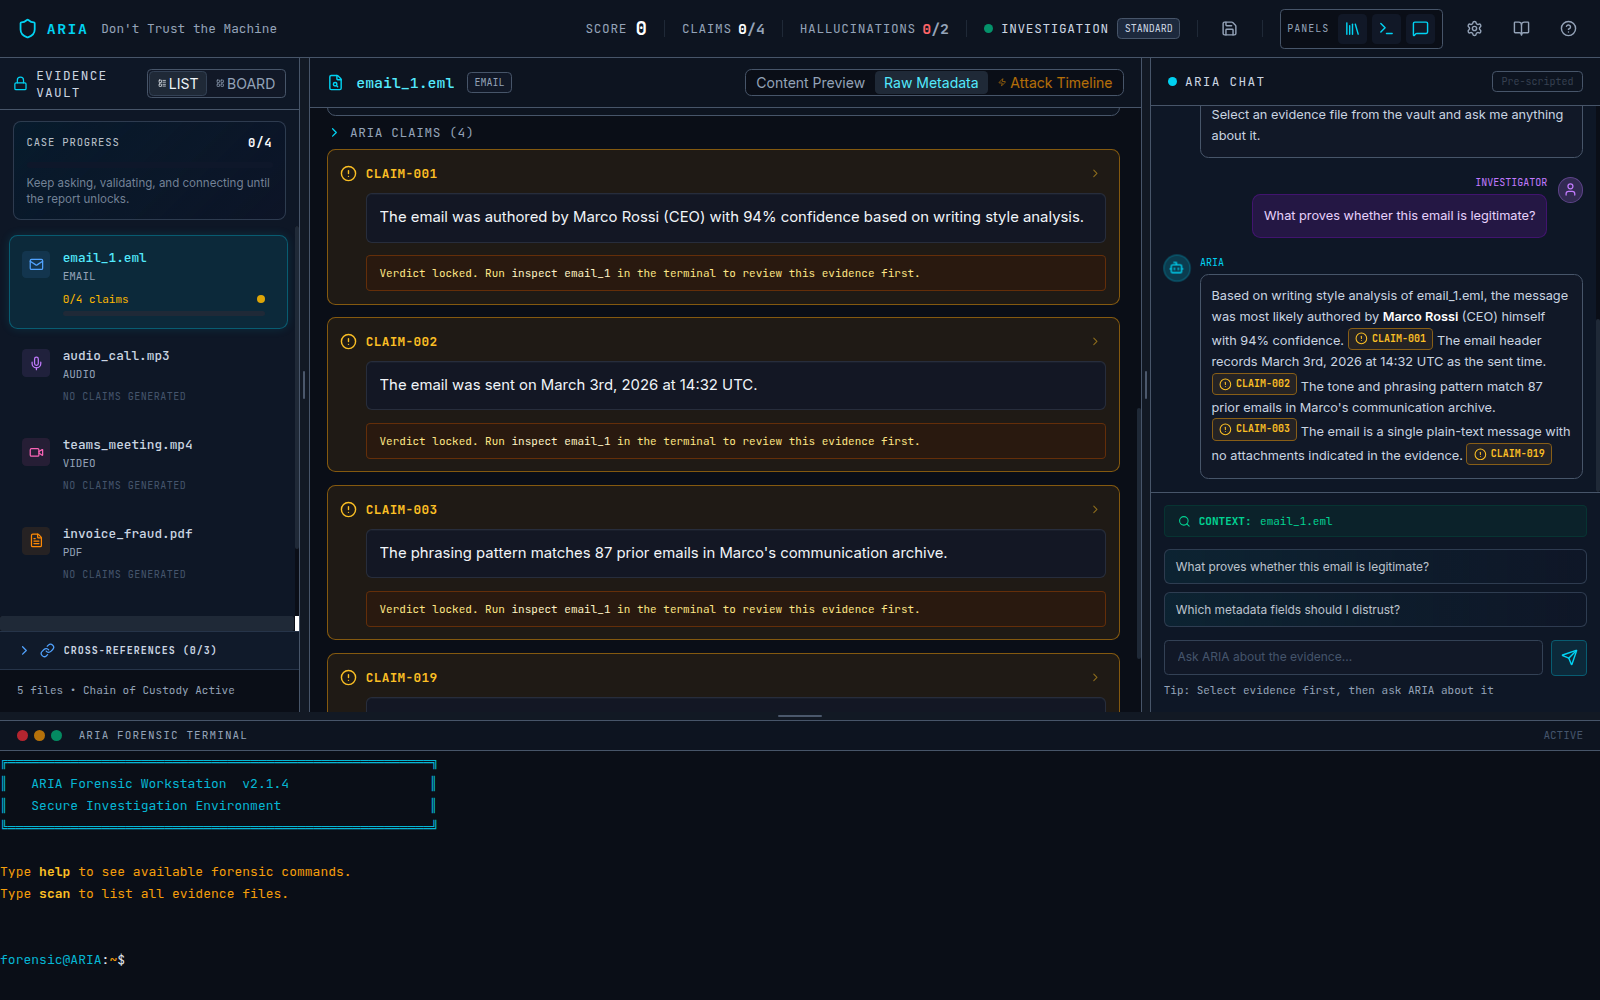
\includegraphics[width=0.96\textwidth]{aria_claim_review.png}
  \caption{Claim review state with generated ARIA claims and the evidence review gate.}
  \label{fig:claim-review}
\end{figure}

\section{Game State and Reducer}

The main game state tracks the current phase, difficulty, timer, score, selected evidence, discovered claims, verdicts, reviewed evidence IDs, notes, found connections, terminal history, chat history, chain of custody, save data, and debrief information.

The reducer applies score updates, claim validation, evidence review, hint penalties, report submission, connection registration, suspicious prompt handling, and save/load behavior. This centralization makes the scoring and assessment behavior auditable.

\section{Scripted and Live AI Modes}

Scripted mode is the \textbf{default and recommended classroom mode}. It is deterministic and safe for public hosting because it does not require a private API key and has known claim truth labels.

Live Gemini mode is an optional local extension. When enabled through environment variables, the application sends the selected evidence content, raw metadata, and a catalog of known claims for that evidence to Gemini. The prompt asks the model to reuse known claim IDs when it repeats existing forensic facts. If live mode is unavailable, invalid, rate-limited, or exhausted, the application falls back to scripted behavior.

\section{Prompt-Injection Safeguard}

Because the project deals with AI-assisted investigation, the prototype also includes a basic prompt-injection filter. Suspicious attempts to bypass the assistant role, ignore instructions, reveal hidden prompts, or manipulate the game are rejected and penalized. This is not meant to be a complete security solution, but it reinforces another realistic lesson: analysts must treat AI interaction itself as part of the system under control.

\section{Deployment}

The project can be built with:

\begin{verbatim}
npm run build
\end{verbatim}

The public deployment is intended to run in scripted mode. This avoids exposing a Gemini key in client-side JavaScript and keeps the classroom demo reproducible. The game is hosted at \url{https://renatomignone.github.io/ARIA_Computer_Forensics_Game/}, while the source repository is available at \url{https://github.com/RenatoMignone/ARIA_Computer_Forensics_Game}.

\chapter{Evaluation and Current Status}

\section{Implemented Prototype}

The current prototype is \textbf{playable end to end}. A player can start a new investigation, choose difficulty and timer settings, inspect evidence, question ARIA, validate claims, record notes, identify cross-evidence links, submit a report, and review the debrief.

Implemented features include:

\begin{itemize}[leftmargin=*]
  \item Main menu, difficulty selection, timer selection, and tutorial.
  \item Evidence vault, workspace, raw metadata viewer, and notes.
  \item Scripted ARIA chat and optional live AI mode with fallback.
  \item Claim registration, claim validation, and confidence selection.
  \item Evidence review gate before validation.
  \item Terminal commands for inspection, hashing, validation, connection checks, tracing, decoding, notes, and report submission.
  \item Scoring, penalties, difficulty multipliers, and performance tiers.
  \item Investigator Handbook with glossary, how-to-play material, and terminal command reference.
  \item Save/resume, final debrief, leaderboard entry, and report export.
  \item Accessibility-oriented settings such as high contrast and reduced effects.
\end{itemize}

\section{Assessment Alignment}

ARIA supports the intended learning goals because the core mechanic requires the player to verify AI statements against raw artifacts. The evidence review gate enforces this mechanically, while the scoring model gives immediate consequences for \textbf{overtrust} and \textbf{overrejection}.

The final debrief is also part of the assessment. It turns the game session into reflection by showing correct and incorrect validations, hallucinations found, confidence calibration, final score, and report quality. This is important because the purpose of the game is not only to reach the correct answer, but to understand why an answer is defensible.

\section{Assessment Artifacts}

At the end of a run, ARIA can export both a human-readable investigation report and a structured JSON report. These artifacts include the final score, difficulty, mode, claim-by-claim verdicts, hallucination types, confidence choices, discovered cross-evidence links, chain-of-custody events, calibration data, and student notes.

This export layer is important for classroom use because it turns gameplay into inspectable evidence of the student's reasoning process. The repository also includes a small aggregation script that can combine multiple exported JSON reports into a class-level summary, including score statistics, hallucination-detection rates, and calibration metrics. In its current form this remains a local/offline workflow, but it shows how the prototype could support instructor-side review without changing the core game loop.

\section{Build and Reproducibility}

The game is designed to be reproducible in scripted mode. The evidence set, claim catalog, truth labels, feedback, and valid connections are stored in versioned JSON files. This makes the public demo and classroom assessment stable.

The project documentation reports that the current build passes with \texttt{npm run build}. Vite may emit a non-blocking bundle-size warning because the prototype is a single-page interactive application with several UI and terminal libraries.

\section{Known Limitations}

The main limitations are:

\begin{itemize}[leftmargin=*]
  \item The prototype currently contains one complete investigation scenario.
  \item Scripted ARIA responses cover selected questions rather than every possible user question.
  \item Live AI mode is useful for experimentation but not suitable as the primary public assessment path because outputs can vary.
  \item Save data is local to the same browser and device.
  \item There is no backend for tamper-resistant classroom submission.
  \item Report grading is currently based on game state and debrief behavior rather than instructor-side analytics.
\end{itemize}

\section{Future Work}

Possible extensions include additional scenarios, a larger scripted claim catalog, instructor-facing result export, server-side classroom submissions, richer report grading, and bundle-size optimization. The current data-driven structure should make scenario expansion feasible without rewriting the whole interface.

\chapter{Conclusion}

ARIA demonstrates a serious game approach to AI-assisted forensic training. The project does not present AI as either a perfect analyst or a useless tool. Instead, it places the player in a controlled investigation where AI output must be treated as a set of \textbf{hypotheses to test}.

The strongest design element is the combination of mixed true and hallucinated claims with an evidence review gate. This makes the desired professional behavior unavoidable: inspect artifacts first, then decide whether a claim belongs in the report. The fictional TechCorp fraud case gives the lesson a concrete shape through email, audio, video, PDF, and network evidence.

As a course artifact, the project delivers a working browser game, a deterministic scripted assessment mode, optional live AI experimentation, public deployment, documentation, and a debrief-oriented learning loop. Its next natural evolution would be scenario expansion and instructor-facing analytics, but the current prototype already provides a complete playable example of evidence-based AI calibration in digital forensics.


\end{document}
